%%%%%%%%%%%%%%%%%%%%%%%%%%%%%%%%%%%%%%%%%
% Beamer Presentation
% LaTeX Template
% Version 1.0 (10/11/12)
%
% This template has been downloaded from:
% http://www.LaTeXTemplates.com
%
% License:
% CC BY-NC-SA 3.0 (http://creativecommons.org/licenses/by-nc-sa/3.0/)
%
%%%%%%%%%%%%%%%%%%%%%%%%%%%%%%%%%%%%%%%%%

%----------------------------------------------------------------------------------------
%	PACKAGES AND THEMES
%----------------------------------------------------------------------------------------
\documentclass{beamer}
\usepackage{subscript}
\usepackage{color}
\usepackage{xcolor}
\usepackage{multimedia}
\usepackage{hyperref}
\usepackage{graphicx}
\usepackage{amsmath}
\usepackage{amsfonts}
\usepackage{amssymb}
\usepackage[makeroom]{cancel}


\mode<presentation> {

% The Beamer class comes with a number of default slide themes
% which change the colors and layouts of slides. Below this is a list
% of all the themes, uncomment each in turn to see what they look like.

%\usetheme{default}
%\usetheme{AnnArbor}
%\usetheme{Antibes}
%\usetheme{Bergen}
%\usetheme{Berkeley}  
%\usetheme{Berlin}
%\usetheme{Boadilla}
%\usetheme{CambridgeUS}	
%\usetheme{Copenhagen}
%\usetheme{Darmstadt}
%\usetheme{Dresden}
%\usetheme{Frankfurt}	
%\usetheme{Goettingen}
\usetheme{Hannover}	% Inhaltsverzeichnis an der linken Seite, hellblau
%\usetheme{Ilmenau}
%\usetheme{JuanLesPins}
%\usetheme{Luebeck}
%\usetheme{Madrid}			%default blau
%\usetheme{Malmoe}
%\usetheme{Marburg}
%\usetheme{Montpellier}
%\usetheme{PaloAlto}				%dunkeblau mit inhaltsverz
%\usetheme{Pittsburgh}   
%\usetheme{Rochester}
%\usetheme{Singapore}
%\usetheme{Szeged}
%\usetheme{Warsaw}

% As well as themes, the Beamer class has a number of color themes
% for any slide theme. Uncomment each of these in turn to see how it
% changes the colors of your current slide theme.

%\usecolortheme{albatross}
%\usecolortheme{beaver}
%\usecolortheme{beetle}
%\usecolortheme{crane}
%\usecolortheme{dolphin}
%\usecolortheme{dove}
%\usecolortheme{fly}
%\usecolortheme{lily}
%\usecolortheme{orchid}
%\usecolortheme{rose}
%\usecolortheme{seagull}
%\usecolortheme{seahorse}
%\usecolortheme{whale}
%\usecolortheme{wolverine}

%\setbeamertemplate{footline} % To remove the footer line in all slides uncomment this line
%\setbeamertemplate{footline}[page number] % To replace the footer line in all slides with a simple slide count uncomment this line

%\setbeamertemplate{navigation symbols}{} % To remove the navigation symbols from the bottom of all slides uncomment this line
}

\usepackage{graphicx} % Allows including images
\usepackage{booktabs} % Allows the use of \toprule, \midrule and \bottomrule in tables

%----------------------------------------------------------------------------------------
%	TITLE PAGE
%----------------------------------------------------------------------------------------

\title[Cross Correlation]{Synchronizing Audio Signals\\ - \\ via Landmark Cross Correlation} % The short title appears at the bottom of every slide, the full title is only on the title page

%		\author{Lea N. Possberg} % Your name
\institute[Uni Bi] % Your institution as it will appear on the bottom of every slide, may be shorthand to save space
{

\textit{by Lea N. Possberg} % Your email address

\medskip

Seminar: Speech Processing \\ % Your institution for the title page




}
\date{November 30, 2017} % Date, can be changed to a custom date

\begin{document}

\begin{frame}
\titlepage % Print the title page as the first slide
\end{frame}


\begin{frame}
\frametitle{Motivation} % Table of contents slide, comment this block out to remove it
%\tableofcontents
%----------------
\begin{figure}
\begin{center}
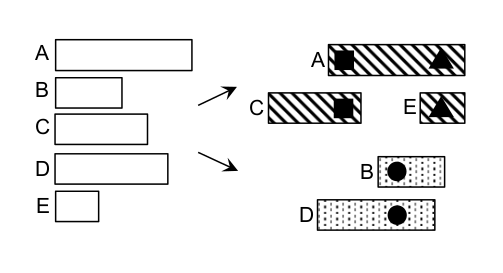
\includegraphics[scale=0.3]{pngs/01_orig_cluster_synch.png} \\
\caption{Clustering and Synchronization (Bryan, Smaragdis, Mysore, 2012)}
\end{center}
\end{figure}
 %---------------
\end{frame}


%----------------------------------------------------------------------------------------
%	PRESENTATION SLIDES
%----------------------------------------------------------------------------------------


%------------------------------------------------
\section{Cross Correlation Function R}
%------------------------------------------------

\subsection{Formula}
\begin{frame}
\frametitle{Cross Correlation Function R}
\begin{displaymath}
R_{f,g}(\tau)= \sum_{ t = -\infty}^{\infty}  f^*(t) g(\tau +t) %HERE!
\end{displaymath}
\end{frame}


\subsection{Demo}
\begin{frame}
\frametitle{What does R do?}
\begin{center}
\movie[height = 0.6\textwidth, width = 0.8\textwidth, poster, showcontrols] {Video}{video/corr.mp4}
\end{center}
(https://www.youtube.com/watch?v=L6YJqhbsuFY) 
\end{frame}


\subsection{Formula with Landmark Signals}
\begin{frame}
\frametitle{Cross Correlation Function R - Landmark Signals}
\begin{displaymath}
R_{f,g}(\tau)= \sum_{ t = -\infty}^{\infty}  f^*(t) g(\tau +t) %HERE!
\end{displaymath}
\end{frame}


\begin{frame}
\frametitle{Cross Correlation Function R - Landmark Signals}
\begin{displaymath}
R_{  \textcolor{green}{f,g}   }(\tau)= \sum_{ t = -\infty}^{\infty}  \textcolor{green}{f}^*(t) \textcolor{green}{g}(\tau +t)
\end{displaymath}
\end{frame}



\begin{frame}
\frametitle{Cross Correlation Function R - Landmark Signals}
\begin{displaymath}
R_{  \textcolor{green}{f,g}   }(\tau)= \sum_{ t = -\infty}^{\infty}  \textcolor{green}{f}^*(t) \textcolor{green}{g}(\tau +t)
\end{displaymath}
\begin{displaymath}
R_{  \textcolor{green}{L_i,L_j}  }(\tau)= \sum_{ t = -\infty}^{\infty}  \textcolor{green}{L_i}(\tau)^T \textcolor{green}{L_j}(\tau +t)
\end{displaymath}
\end{frame}



\begin{frame}
\frametitle{Cross Correlation Function R - Landmark Signals}
\begin{displaymath}
R_{  \textcolor{green}{f,g}   }(\tau)= \sum_{ t = -\infty}^{\infty}  \textcolor{green}{f} ^*(t) \textcolor{green}{g}(\tau +t)
\end{displaymath}
\begin{displaymath}
R_{  \textcolor{green}{L_i,L_j}  }(\tau)= \sum_{ t = -\infty}^{\infty}   \textcolor{green}{L_i}(t)\textcolor{red}{^T} \textcolor{green}{L_j}(\tau +t)
\end{displaymath}
\end{frame}



%\begin{frame}
%\frametitle{Cross Correlation Function R - Landmark Signals}
%\begin{displaymath}
%R_{  L_i,L_j  }(\tau)= \sum_{ t = -\infty}^{\infty}  L_i(t)^T L_j(\tau +t)
%\end{displaymath}
%\end{frame}



\begin{frame}
\frametitle{Landmark Signals - Why?}
%----------------
\begin{figure}
\begin{center}
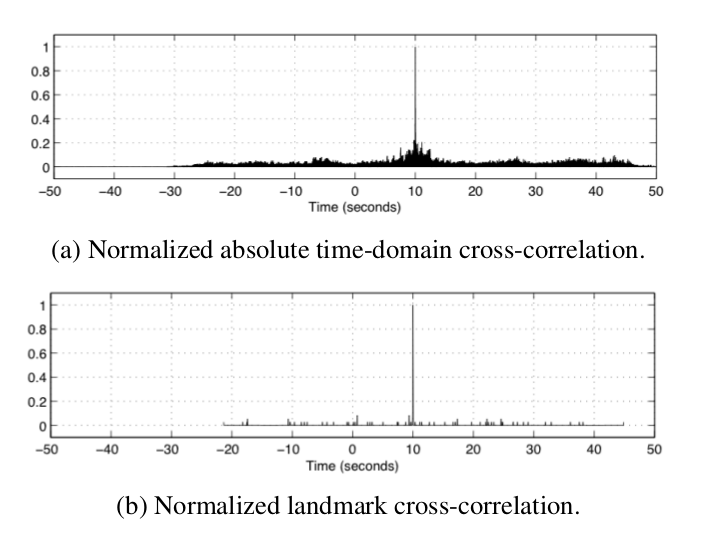
\includegraphics[scale=0.23]{pngs/02_absolute_vs_landmark.png} \\
\caption{Absolute vs. Landmark Cross Correlation (Bryan, Smaragdis, Mysore, 2012)}
\end{center}
\end{figure}
 %---------------
\end{frame}


%------------------------------------------------
\section{Generating Landmark Signals}
\begin{frame}
\frametitle{Generating Landmark Signals - How?}
\begin{center}
Follow Steps 1-4
\end{center}
\end{frame}

%------------------------------------------------
\subsection{1. STFT}
\begin{frame}
\frametitle{1. Take the Short Time FT of a given audio signal}
\begin{columns}
\column{0.475\textwidth}
\begin{figure}
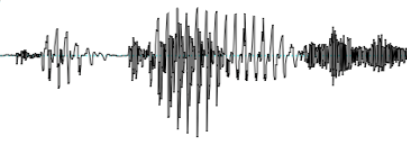
\includegraphics[scale=0.25]{pngs/03_oszillo.png} 
\caption{Given audio signal}
\end{figure}
\column{0.05\textwidth}
$\xrightarrow[]{\text{STFT}}$
\column{0.475\textwidth}
\begin{figure}
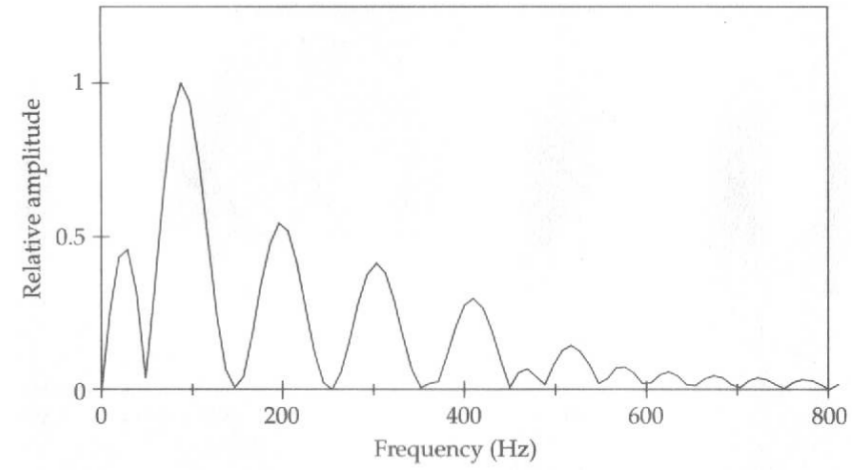
\includegraphics[scale=0.1]{pngs/04_spektrum.png} 
\caption{Spectrum}
\end{figure}
\end{columns}
\ \\
\ \\
\ \\
\ \\
\ \\
\ \\
(Images: Wagner, 2017)
\end{frame}


\subsection{2. Create Landmarks}
\begin{frame}
\frametitle{2. Identify frequency peaks and create landmark tuple}
\begin{columns}
\column{0.475\textwidth}
\begin{figure}
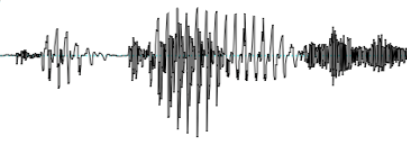
\includegraphics[scale=0.25]{pngs/03_oszillo.png} 
\caption{Given audio signal}
\end{figure}
\column{0.05\textwidth}
$\xrightarrow[]{\text{STFT}}$
\column{0.475\textwidth}
\begin{figure}
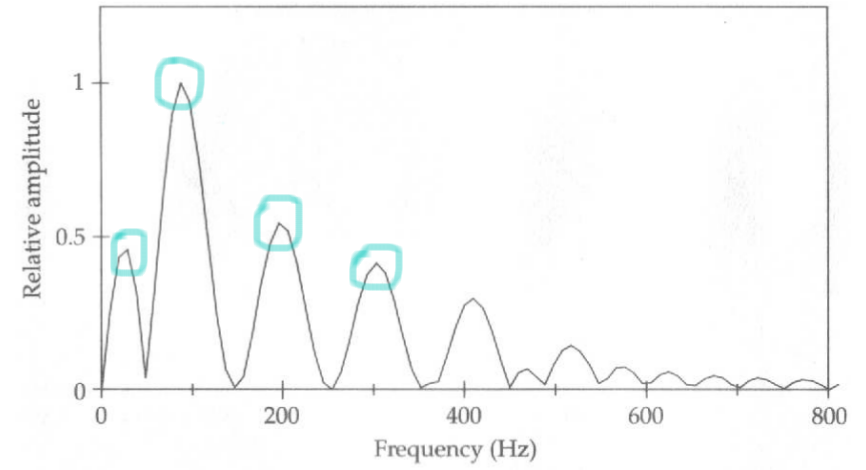
\includegraphics[scale=0.1]{pngs/05_spektrum.png} 
\caption{Spectrum}
\end{figure}
\end{columns}
\ \\
\ \\
\ \\
\ \\
\ \\
\ \\
(Images: Wagner, 2017)
\end{frame}


\begin{frame}
\frametitle{2. Identify frequency peaks and create landmark tuple}
\begin{figure}
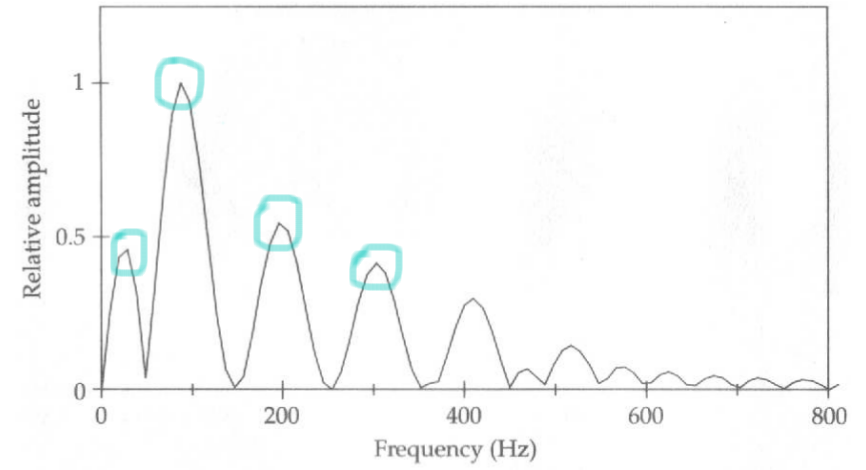
\includegraphics[scale=0.1]{pngs/05_spektrum.png} 
\caption{Spectrum}
\end{figure}
\begin{center}
landmark = (frequency, timevalue) = $(f_1, t_1)$\\
\ \\
"time idexed frequency value"
\end{center}
\end{frame}



\begin{frame}
\begin{columns}
\column{0.5\textwidth}
\frametitle{2. Identify frequency peaks and create landmark tuple}
\begin{figure}
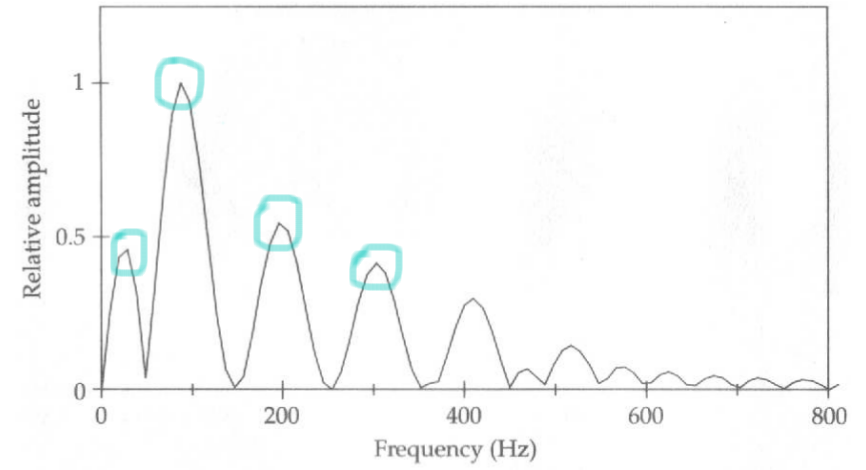
\includegraphics[scale=0.1]{pngs/05_spektrum.png} 
\caption{Spectrum}
\end{figure}
\begin{center}
landmark = $(f_1, t_1)$\\
\end{center}
\column{0.5\textwidth}
\begin{figure}
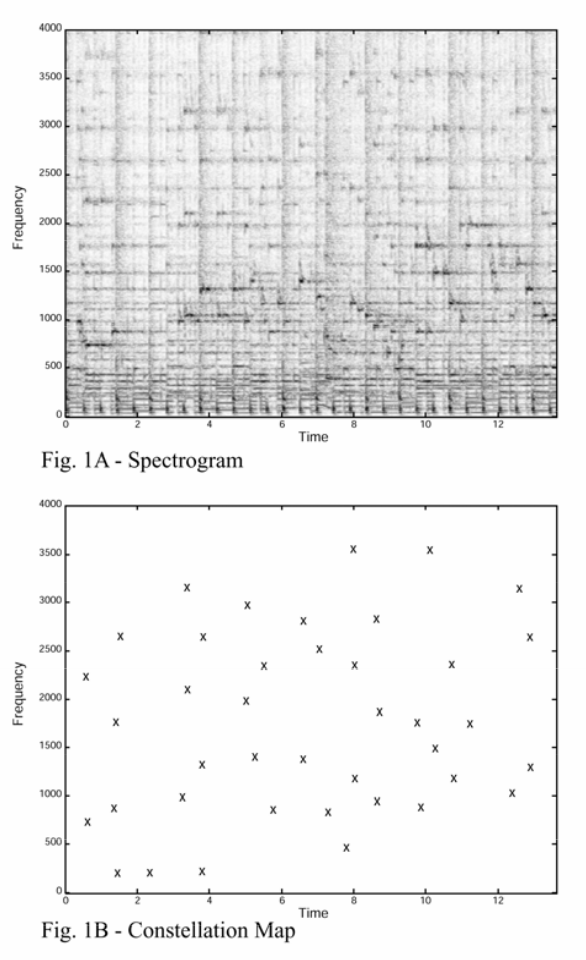
\includegraphics[scale=0.14]{pngs/06_spektrogramm.png} 
\caption{Spectrogram (Wang, 2003)}
\end{figure}
\end{columns}
\end{frame}




\subsection{3. Pair Landmarks}
\begin{frame}
\frametitle{3. Pair landmarks with nearest other landmarks}
\begin{figure}
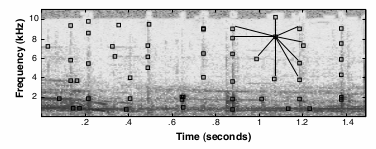
\includegraphics[scale=0.5]{pngs/07_spektrogramm.png} 
\caption{Spectrogram (Kennedy, Naaman, 2009)}
\end{figure}
\end{frame}


\begin{frame}
\frametitle{3. Pair landmarks with nearest other landmarks}
\begin{figure}
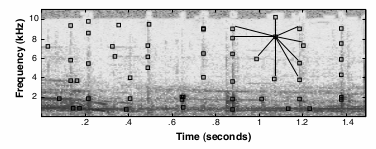
\includegraphics[scale=0.5]{pngs/07_spektrogramm.png} 
\caption{Spectrogram (Kennedy, Naaman, 2009)}
\end{figure}
\begin{center}
landmark-pair = landmark = (frequency, frequency, timevalue) = $(f_1, f_2, t_2-t_1)$\\
\ \\
"time indexed landmark"
\end{center}
\end{frame}






\subsection{4. Hash Landmarks}

\begin{frame}
\frametitle{4. Hash each landmark and create feature vector}
\begin{displaymath}
hash: landmark \rightarrow integer 
\end{displaymath}
\begin{displaymath}
(f_1, f_2, t_2-t_1) \mapsto 2
\end{displaymath}
\end{frame}



\begin{frame}
\frametitle{4. Hash each landmark and create feature vector}
\begin{displaymath}
hash: landmark \rightarrow integer 
\end{displaymath}
\begin{displaymath}
(f_1, f_2, t_2-t_1) \mapsto 2
\end{displaymath}
\ \\
\ \\
create feature vector: $\left( \begin{array}{c}
0\\
0\\
...\\
0\\
\end{array}
\right)$
\end{frame}


\begin{frame}
\frametitle{4. Hash each landmark and create feature vector}
\begin{displaymath}
hash: landmark \rightarrow integer 
\end{displaymath}
\begin{displaymath}
(f_1, f_2, t_2-t_1) \mapsto 2
\end{displaymath}
\ \\
\ \\
create feature vector: $\left( \begin{array}{c}
0\\
0\\
...\\
0\\
\end{array}
\right)
\rightarrow
\left( \begin{array}{c}
0\\
1\\
...\\
0\\
\end{array}
\right)
=
L(t=6)
$
\end{frame}




\begin{frame}
\frametitle{4. Hash each landmark and create feature vector}
\begin{displaymath}
hash: landmark \rightarrow integer 
\end{displaymath}
\begin{displaymath}
(f_1, f_2, t_2-t_1) \mapsto 2
\end{displaymath}
\ \\
\ \\
create feature vector: $\left( \begin{array}{c}
0\\
0\\
...\\
0\\
\end{array}
\right)
\rightarrow$
\fcolorbox{red}{white}{
$\left( \begin{array}{c}
0\\
1\\
...\\
0\\
\end{array}
\right)
=
L(t=6)
$
}
\end{frame}




%------------------------------------------------
\section{Understanding R}
%------------------------------------------------

\begin{frame}
\frametitle{Understanding R}
\begin{center}
\fcolorbox{red}{white}{
$\left( \begin{array}{c}
0\\
1\\
...\\
0\\
\end{array}
\right)
=
L(t=6)
$
}
\end{center}
\ \\
\ \\
\begin{displaymath}
R_{  L_i,L_j  }(\tau)= \sum_{ t = -\infty}^{\infty}  L_i(t)^T L_j(\tau +t)
\end{displaymath}
\end{frame}



\begin{frame}
\frametitle{Understanding R}
\begin{displaymath}
R_{  L_i,L_j  }(\tau)=  \sum_{t = -\infty}^{\infty} \textcolor{green}{ \underbrace{ \textcolor{black}{ L_i(t)^T L_j(\tau +t)} }}
\end{displaymath}
\ \\
\ \\
\begin{center}
\textcolor{green}{
$
\begin{pmatrix}
0 & 1 & ... & 0 \\
\end{pmatrix}
\left( \begin{array}{c}
0\\
0\\
...\\
1\\
\end{array}
\right)
= constant
$
}
\end{center}
\end{frame}




\begin{frame}
\frametitle{Understanding R}
\begin{displaymath}
R_{  L_i,L_j  }(\tau)=  \sum_{t = -\infty}^{\infty} \textcolor{green}{ \underbrace{ \textcolor{black}{ L_i(t)^T L_j(\tau +t)} }}
\end{displaymath}
\ \\
\ \\
\begin{center}
\textcolor{green}{
$
\begin{pmatrix}
0 & 1 & ... & 0 \\
\end{pmatrix}
\left( \begin{array}{c}
0\\
0\\
...\\
1\\
\end{array}
\right)
= constant
$
}
\ \\
\ \\
\textcolor{green}{"Amout of matching landmarks in both signals at one point in time"}
\end{center}
\end{frame}




\begin{frame}
\frametitle{Understanding R}
\begin{displaymath}
R_{  L_i,L_j  }(\tau)=  \textcolor{blue}{  \sum_{t = -\infty}^{\infty} \textcolor{green}{ \underbrace{ \textcolor{black}{ L_i(t)^T L_j(\tau +t)} }}}
\end{displaymath}
\ \\
\ \\
\begin{center}
\textcolor{green}{
$
\begin{pmatrix}
0 & 1 & ... & 0 \\
\end{pmatrix}
\left( \begin{array}{c}
0\\
0\\
...\\
1\\
\end{array}
\right)
= constant
$
}
\ \\
\ \\
\textcolor{green}{"Amout of matching landmarks in both signals at one point in time"}
\ \\
\ \\
\textcolor{blue}{"Total amount of matching landmarks for one time shift $\tau$"}
\end{center}
\end{frame}




\begin{frame}
\frametitle{Understanding R}
\begin{center}
\movie[height = 0.6\textwidth, width = 0.8\textwidth, poster, showcontrols] {Video}{corr.mp4}
\end{center}
(https://www.youtube.com/watch?v=L6YJqhbsuFY) 
\end{frame}



%------------------------------------------------
\section{Synchronizing two files}
%------------------------------------------------
\begin{frame}
\frametitle{Synchronizing both signals}
\begin{displaymath}
\hat{\tau}_{ij} = arg \max_{\tau} R_{L_{i}, L_{j}} (\tau)
\end{displaymath}
\end{frame}


\begin{frame}
\frametitle{Synchronizing both signals}
\begin{displaymath}
\textcolor{green}{
\hat{\tau}_{ij} } = arg \max_{\tau} R_{L_{i}, L_{j}} (\tau)
\end{displaymath}
\ \\
\ \\
\begin{center}
\textcolor{green}{
"time offset to align both signals $L_i$ and $L_j$"
}
\end{center}
\end{frame}







%------------------------------------------------
\section{Complexity}
%------------------------------------------------
\begin{frame}
\frametitle{Complexity \ \\ ($n$ $\hat{=}$ $file$ $length$)}
\begin{itemize}
\item 2 loops over $t$, $\tau$ \ \ $\longrightarrow$ \ \ \textbf{O(n$^2$)}
\end{itemize}
\end{frame}

\begin{frame}
\frametitle{Complexity \ \\ ($n$ $\hat{=}$ $file$ $length$)}
\begin{itemize}
\item 2 loops over $t$, $\tau$ \ \ $\longrightarrow$ \ \ \textbf{O(n$^2$)}
\ \\
\ \\
\item use FFT: no need to loop over $t$ anymore,\\ only 1 loop over $\tau$ \ \ $\longrightarrow$ \ \ \textbf{O(n log n)}
\end{itemize}
\end{frame}



\subsection{FFT of signals}

\begin{frame}
\frametitle{FFT of the two signals}
\begin{displaymath}
R_{f,g}(\tau)= \sum_{ t = -\infty}^{\infty}  f^*(t) g(\tau +t) %HERE!
\end{displaymath}
\end{frame}


\begin{frame}
\frametitle{FFT of the two signals}
\begin{displaymath}
R_{f,g}(\tau)= \sum_{ t = -\infty}^{\infty} \textcolor{orange}{  f^*(t)} g(\tau +t) %HERE!
\end{displaymath}
\ \\
\ \\
\ \\
Frequency Domain:  \ \ \ \ \ \ \ \ \ \ \ 
\textcolor{orange}{$FFT(f^*)$} 
\end{frame}


\begin{frame}
\frametitle{FFT of the two signals}
\begin{displaymath}
R_{f,g}(\tau)= \sum_{ t = -\infty}^{\infty} \textcolor{orange}{  f^*(t) g(\tau +t) }%HERE!
\end{displaymath}
\ \\
\ \\
\ \\
Frequency Domain:  \ \ \ \ \ \ \ \ \ \ \ 
\textcolor{orange}{$FFT(f^*)$ \ $FFT(g)$} 
\end{frame}


\begin{frame}
\frametitle{FFT of the two signals}
\begin{displaymath}
R_{f,g}(\tau)= \sum_{ t = -\infty}^{\infty} \textcolor{orange}{  f^*(t) g(\tau +t) }%HERE!
\end{displaymath}
\ \\
\ \\
\ \\
Frequency Domain:  \ \ \ \ \ \ \ \ \ \ \ 
\textcolor{orange}{$FFT(f^*)$ \textbf{$*$} $FFT(g)$} 
\end{frame}


\begin{frame}
\frametitle{FFT of the two signals}
\begin{displaymath}
R_{f,g}(\tau)= \sum_{ t = -\infty}^{\infty} \textcolor{orange}{  f^*(t) g(\tau +t) }%HERE!
\end{displaymath}
\ \\
\ \\
\ \\
Frequency Domain:  \ \ \ \ \ \ \ \ \ \ \ 
\textcolor{orange}{$FFT(f^*)$ \textbf{$*$} $FFT(g)$} 
\ \\
\ \\
\ \\
Time Domain: \ \ \ \ \ \ \ \  IFFT ( \textcolor{orange}{$FFT(f^*)$ \textbf{$*$} $FFT(g)$} )
\end{frame}


\begin{frame}
\frametitle{FFT of the two signals}
\begin{displaymath}
R_{f,g}(\tau)= \xcancel{ \sum_{ t = -\infty}^{\infty} } \textcolor{orange}{  f^*(t) g(\tau +t) }%HERE!
\end{displaymath}
\ \\
\ \\
\ \\
Frequency Domain:  \ \ \ \ \ \ \ \ \ \ \ 
\textcolor{orange}{$FFT(f^*)$ \textbf{$*$} $FFT(g)$} 
\ \\
\ \\
\ \\
Time Domain: \ \ \ \ \ \ \ \  IFFT ( \textcolor{orange}{$FFT(f^*)$ \textbf{$*$} $FFT(g)$} )
\end{frame}




%------------------------------------------------
\section{Summary}
%------------------------------------------------
\begin{frame}
\frametitle{Take home}
\begin{enumerate}
\item $R_{f,g}(\tau)= \sum_{ t = -\infty}^{\infty}  f^*(t) g(\tau +t)$ %HERE!
\end{enumerate}
\end{frame}

\begin{frame}
\frametitle{Take home}
\begin{enumerate}
\item $R_{f,g}(\tau)= \sum_{ t = -\infty}^{\infty}  f^*(t) g(\tau +t)$ %HERE!
\ \\
\ \\
\item Reduce costs by transforming absolute signals $f, g$ to Landmark signals $L_i, L_j$
\end{enumerate}
\end{frame}

\begin{frame}
\frametitle{Take home}
\begin{enumerate}
\item $R_{f,g}(\tau)= \sum_{ t = -\infty}^{\infty}  f^*(t) g(\tau +t)$ %HERE!
\ \\
\ \\
\item Reduce costs by transforming absolute signals $f, g$ to Landmark signals $L_i, L_j$
\ \\
\ \\
\item Reduce complexity by applying the FFT to both signals before multiplying them, then apply IFFT to the result
\end{enumerate}
\end{frame}





%------------------------------------------------
\section{Sources}
\begin{frame}
\frametitle{Sources}

"Clustering and Synchronizing Multi-Camera Video via Landmark Cross-Correlation", Bryan, Smaragdis, Mysore, 2012\\
\ \\
https://www.youtube.com/watch?v=L6YJqhbsuFY \\
\ \\
Wagner, 2017 (Lecture "Phonetik und Phonologie" Slides "Akustische Phonetik")\\
\ \\
"An Industrial-Strength Audio Search Algorithm", Wang, 2003\\
\ \\
"Less Talk, More Rock: Automated Organization of Community-Contributed Collections of Concert Videos", Kennedy and Naaman, 2009 \\
\ \\


\end{frame}
%------------------------------------------------










	 


\end{document} 